\documentclass[answers]{exam}

\usepackage{color} 
\usepackage[table,svgnames]{xcolor}
\usepackage{lstautogobble, listings} 

\usepackage{tikz}
\usepackage{float}

\usetikzlibrary{automata, positioning, arrows}

\definecolor{bluekeywords}{rgb}{0.13, 0.19, 0.7}
\definecolor{goldenkeywords}{rgb}{0.67, 0.58, 0.13}
\definecolor{greencomments}{rgb}{0.1, 0.5, 0.2}
\definecolor{redstrings}{rgb}{0.8, 0.15, 0.1}
\definecolor{graynumbers}{rgb}{0.5, 0.5, 0.5}
\definecolor{subtlegray}{rgb}{0.98, 0.98, 0.98}

\lstset{
    autogobble,    
    columns=fullflexible,
    showspaces=false,
    showtabs=false,
    breaklines=true,
    showstringspaces=false,
    numbers=left,
    breakatwhitespace=true,
    escapeinside={(*@}{@*)},
    rulecolor=\color{lightgray},
    backgroundcolor=\color{subtlegray},
    commentstyle=\color{greencomments},
    keywordstyle=\color{bluekeywords},
    ndkeywordstyle=\color{goldenkeywords},
    stringstyle=\color{redstrings},
    numberstyle=\color{graynumbers},
    basicstyle=\ttfamily\linespread{1.15}\footnotesize,
    frame=tb,
    framesep=12pt,
    framexleftmargin=12pt,
    tabsize=4,
    captionpos=b
}

\lstdefinelanguage{TML}{ 
    keywords={changeto, move, goto, if, switch, while, module, accept, reject, halt, alphabet},
    ndkeywords={left, right, tapehead, blank},
    sensitive=true,
    comment=[l]{//},
    morecomment=[s]{/*}{*/},
    morestring=[b]',
    morestring=[b]"
}

\begin{document}
    % \addtitle{TML Worksheet}
    \section{Introduction to Turing Machine Language}
    In this section, you are given some programs in Turing Machine Language (TML). They will be used to explain the syntax of the programming language and how they can be run on tapes.
    \begin{itemize}
        \item \texttt{isDiv2}:
        \lstinputlisting[language=TML]{code/isDiv2.tm}
        
        \item \texttt{isDiv2Rec}:
        \lstinputlisting[language=TML]{code/isDiv2Rec.tm}

        \noindent Both \texttt{isDiv2} and \texttt{isDiv2Rec} correspond to the following Turing Machine (TM):
        \begin{figure}[H]
            \centering
            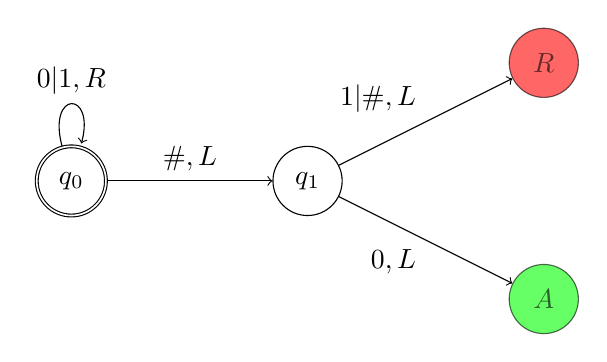
\begin{tikzpicture}
                \node[state, accepting] (q0) at (0, 0) {$q_0$};
                \node[state] (q1) at (3, 0) {$q_1$};
                \node[state, fill=green, opacity=0.6] (A) at (6, -1.5) {$A$};
                \node[state, fill=red, opacity=0.6] (R) at (6, 1.5) {$R$};

                \draw[->] (q0) edge[loop above] node {$0|1, R$} (q0);
                \draw[->] (q0) -- node[above] {$\#, L$} (q1);
                \draw[->] (q1) -- node[below left] {$0, L$} (A);
                \draw[->] (q1) -- node[above left] {$1|\#, L$} (R);
            \end{tikzpicture}
        \end{figure}
        \newpage
        
        \item \texttt{palindrome}:
        \lstinputlisting[language=TML]{code/palindrome.tm}

        \noindent The program \texttt{palindrome} corresponds to the following TM:
        \begin{figure}[H]
            \centering
            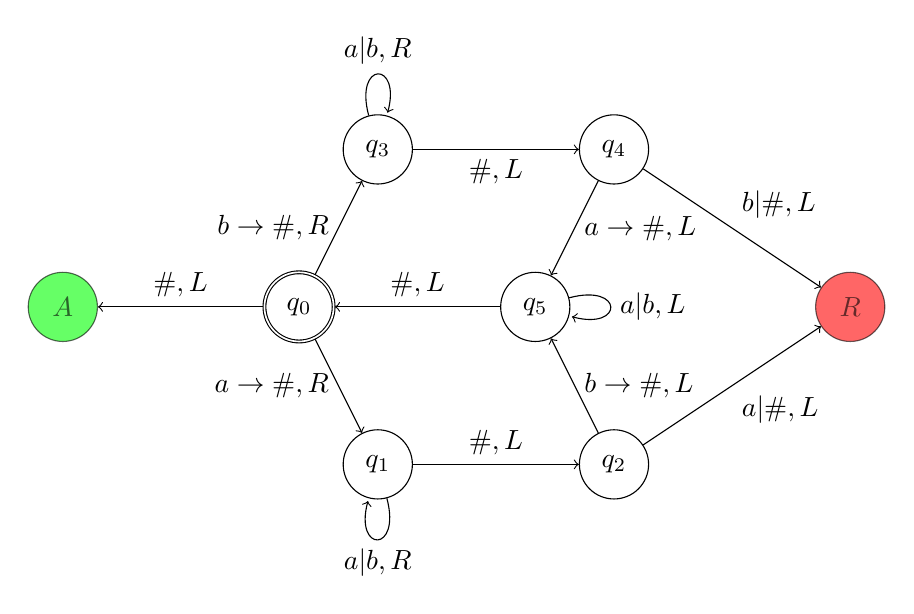
\begin{tikzpicture}
                \node[state, accepting] (q0) at (1, 0) {$q_0$};
                \node[state] (q1) at (2, -2) {$q_1$};
                \node[state] (q2) at (5, -2) {$q_2$};
                \node[state] (q4) at (2, 2) {$q_3$};
                \node[state] (q5) at (5, 2) {$q_4$};
                \node[state] (q7) at (4, 0) {$q_5$};
                \node[state, fill=green, opacity=0.6] (A) at (-2, 0) {$A$};
                \node[state, fill=red, opacity=0.6] (R) at (8, 0) {$R$};
    
                \draw[->] (q0) -- node[left] {$a \to \#, R$} (q1);
                \draw[->] (q0) -- node[left] {$b \to \#, R$} (q4);
                \draw[->] (q0) -- node[above] {$\#, L$} (A);
                \draw[->] (q1) edge[loop below] node {$a|b, R$} (q1);
                \draw[->] (q1) -- node[above] {$\#, L$} (q2);
                \draw[->] (q2) -- node[right] {$b \to \#, L$} (q7);
                \draw[->] (q2) -- node[below right] {$a|\#, L$} (R);
                \draw[->] (q4) edge[loop above] node {$a|b, R$} (q4);
                \draw[->] (q4) -- node[below] {$\#, L$} (q5);
                \draw[->] (q5) -- node[right] {$a \to \#, L$} (q7);
                \draw[->] (q5) -- node[above right] {$b|\#, L$} (R);
                \draw[->] (q7) edge[loop right] node {$a|b, L$} (q7);
                \draw[->] (q7) -- node[above] {$\#, L$} (q0);
                % \draw[->] (q0) -- node[left] {$a \to \#, R$} (q1);
                % \draw[->] (q0) -- node[left] {$b \to \#, R$} (q4);
                % \draw[->] (q0) -- node[above] {$\#, L$} (A);
                % \draw[->] (q1) edge[loop above] node {$a|b, R$} (q1);
                % \draw[->] (q1) -- node[above] {$\#, L$} (q2);
                % \draw[->] (q2) -- node[right] {$b \to \#, L$} (q7);
                % \draw[->] (q2) -- node[right] {$a|\#, L$} (R);
                % \draw[->] (q4) edge[loop below] node {$a|b, R$} (q4);
                % \draw[->] (q4) -- node[below] {$\#, L$} (q5);
                % \draw[->] (q5) -- node[right] {$a \to \#, L$} (q7);
                % \draw[->] (q5) -- node[right] {$b|\#, L$} (R);
                % \draw[->] (q7) edge[loop right] node {$a|b, L$} (q7);
                % \draw[->] (q7) -- node[above] {$\#, L$} (q0);
            \end{tikzpicture}
        \end{figure}

% \begin{lstlisting}[language=TML]
% // checks whether the input is blank or of the form ab, aabb, aaabbb, etc.
% alphabet = {a, b}
% module aNbN {
%     if blank {
%         accept
%     } 
%     // cannot start with a b
%     if b {
%         reject
%     } if a {
%         changeto blank
%         move right
%         // go to the end
%         while a, b {
%             move right
%         } 
%         if blank {
%             move left
%             // must end with a b
%             if a, blank {
%                 reject
%             } if b {
%                 changeto blank
%                 move left
%                 // go to the start and restart
%                 while a, b {
%                     move left
%                 } if blank {
%                     move right
%                     goto aNbN
%                 }
%             }
%         }
%     }
% }
% \end{lstlisting}
    \end{itemize}
    \newpage
    
    \section{Identifying TML Programs}
    In this section, you are presented with TML programs. You will be given some tape values to run the program in and decode what values the program accepts. You are encouraged to use the website to try and solve this.

    \begin{enumerate}
        \item Consider the following TML Program:
        \lstinputlisting[language=TML]{code/mystery1.tm}

        \begin{enumerate}
            \item Does the program accept the values:
            \begin{enumerate}
                \item $2 = 10$
                \begin{solution}
                    
                \end{solution}
                
                \item $1 = 1$
                \begin{solution}
                    
                \end{solution}
                
                \item $4 = 100$
                \begin{solution}
                    
                \end{solution}
                
                \item $5 = 101$
                \begin{solution}
                    
                \end{solution}
                
                \item $6 = 110$
                \begin{solution}
                    
                \end{solution}
            \end{enumerate}
            
            \item Describe the values this program accepts.
            \begin{solution}
                \vspace*{30pt}
            \end{solution}
        \end{enumerate}
        \newpage

        \item Consider the following TML program:
        \lstinputlisting[language=TML]{code/mystery2.tm}
        \begin{enumerate}
            \item Does the program accept the values:
            \begin{enumerate}
                \item $ab$
                \begin{solution}
                    
                \end{solution}
                \newpage
                
                \item $aab$
                \begin{solution}
                    
                \end{solution}
                
                \item $abb$
                \begin{solution}
                    
                \end{solution}
                
                \item $abba$
                \begin{solution}
                    
                \end{solution}
                
                \item $abab$
                \begin{solution}
                    
                \end{solution}
            \end{enumerate}
            
            \item Describe the values this program accepts.
            \begin{solution}
                \vspace*{30pt}
            \end{solution}
        \end{enumerate}
    \end{enumerate}
    
    \newpage

    \section{Identifying TMs}
    In this section, you are presented with TMs. You will be given some tape values to run the program in and decode what values the program accepts. Since the website can only execute TML programs, you are also given the TML program for the code, but it is not comprehensible like the previous programs; you will likely find it easier to understand the TM than the program (which you should do!). 
    \begin{enumerate}
        \item Consider the following TM FSM:
        \begin{figure}[H]
            \centering
            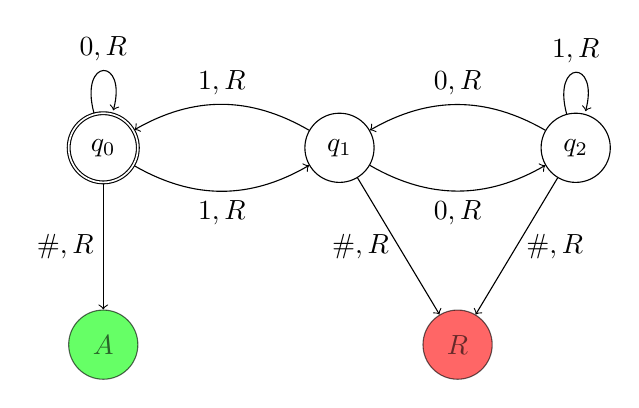
\begin{tikzpicture}
                \node[state, accepting] (q0) at (0, 0) {$q_0$};
                \node[state] (q1) at (3, 0) {$q_1$};
                \node[state] (q2) at (6, 0) {$q_2$};
                \node[state, fill=green, opacity=0.6] (A) at (0, -2.5) {$A$};
                \node[state, fill=red, opacity=0.6] (R) at (4.5, -2.5) {$R$};
    
                \draw[->] (q0) edge[loop above] node {$0, R$} (q0);
                \draw[->] (q0) edge[bend right] node[below] {$1, R$} (q1);
                \draw[->] (q1) edge[bend right] node[above] {$1, R$} (q0);
                \draw[->] (q1) edge[bend right] node[below] {$0, R$} (q2);
                \draw[->] (q2) edge[bend right] node[above] {$0, R$} (q1);
                \draw[->] (q2) edge[loop above] node {$1, R$} (q2);
                \draw[->] (q0) edge node[left] {$\#, R$} (A);
                \draw[->] (q1) edge node[left] {$\#, R$} (R);
                \draw[->] (q2) edge node[right] {$\#, R$} (R);
            \end{tikzpicture}
        \end{figure}
        You are given a basic representation of this FSM as code in Teams.
        \begin{enumerate}
            \item Does the TM accept the values:
            \begin{enumerate}
                \item $2 = 10$
                \begin{solution}
                    
                \end{solution}
                
                \item $1 = 1$
                \begin{solution}
                    
                \end{solution}
                
                \item $6 = 100$
                \begin{solution}
                    
                \end{solution}
                
                \item $5 = 101$
                \begin{solution}
                    
                \end{solution}
                
                \item $8 = 110$
                \begin{solution}
                    
                \end{solution}
            \end{enumerate}
            
            \item Describe the values this program accepts.
            \begin{solution}
                \vspace*{30pt}
            \end{solution}
        \end{enumerate} 
        \newpage   
        
        \item Consider the following TM FSM:
        \begin{figure}[H]
            \centering
            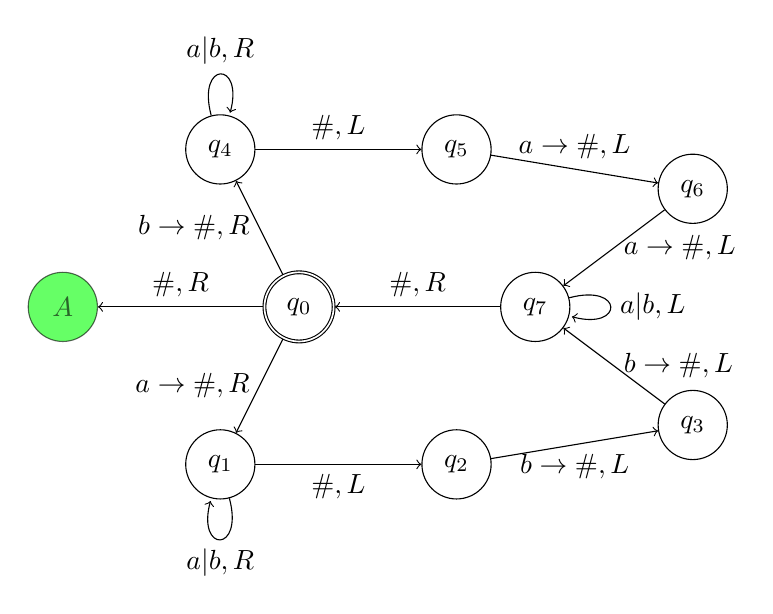
\begin{tikzpicture}
                \node[state, accepting] (q0) at (3, 0) {$q_0$};
                \node[state] (q1) at (2, -2) {$q_1$};
                \node[state] (q2) at (5, -2) {$q_2$};
                \node[state] (q3) at (8, -1.5) {$q_3$};
                \node[state] (q4) at (2, 2) {$q_4$};
                \node[state] (q5) at (5, 2) {$q_5$};
                \node[state] (q6) at (8, 1.5) {$q_6$};
                \node[state] (q7) at (6, 0) {$q_7$};
                \node[state, fill=green, opacity=0.6] (A) at (0, 0) {$A$};
    
                \draw[->] (q0) -- node[left] {$a \to \#, R$} (q1);
                \draw[->] (q0) -- node[left] {$b \to \#, R$} (q4);
                \draw[->] (q0) -- node[above] {$\#, R$} (A);
                \draw[->] (q1) edge[loop below] node {$a|b, R$} (q1);
                \draw[->] (q1) -- node[below] {$\#, L$} (q2);
                \draw[->] (q2) -- node[below] {$b \to \#, L$} (q3);
                \draw[->] (q3) -- node[right] {$b \to \#, L$} (q7);
                \draw[->] (q4) edge[loop above] node {$a|b, R$} (q4);
                \draw[->] (q4) -- node[above] {$\#, L$} (q5);
                \draw[->] (q5) -- node[above] {$a \to \#, L$} (q6);
                \draw[->] (q6) -- node[right] {$a \to \#, L$} (q7);
                \draw[->] (q7) edge[loop right] node {$a|b, L$} (q7);
                \draw[->] (q7) -- node[above] {$\#, R$} (q0);
            \end{tikzpicture}
        \end{figure}
        NOTE: The missing transitions go to the reject state, i.e. $q_2$, $q_3$ to $a|\#$ and $q_5$, $q_6$ to $b|\#$ are rejected. You are given a basic representation of this FSM as code in Teams.
        \begin{enumerate}
            \item Does this TM accept the values:
            \begin{enumerate}
                \item $ab$
                \begin{solution}
                    
                \end{solution}

                \item $abb$
                \begin{solution}
                    
                \end{solution}

                \item $aabb$
                \begin{solution}
                    
                \end{solution}
                
                \item $bbaaaa$
                \begin{solution}
                    
                \end{solution}

                \item $abba$
                \begin{solution}
                    
                \end{solution}

                \item $abab$
                \begin{solution}
                    
                \end{solution}
            \end{enumerate}

            \item Describe the values this program accepts.
            \begin{solution}
                \vspace*{25pt}
            \end{solution}
        \end{enumerate}
    \end{enumerate}
    % Checks isDiv4
    \newpage

    
    \section{Writing TML Programs}
    % In this section, you will be tested on writing TML programs. Three programs are given below as examples:
    
    Following a similar syntax to the code given above, write the following programs. You are free to use the website to check the accuracy of the program while writing the programs.
    \begin{enumerate}
        \item divisibility by 4 in binary iteratively [HINT: Go to the end and check for 2 zeros. Allow 0 as well.]
        \begin{solution}
            \vspace*{520pt}
        \end{solution}
        
        \item divisibility by 4 in binary, recursively.
        \begin{solution}
            \vspace*{570pt}
        \end{solution}
        
        \item check all $a$'s come before the $b$'s
        \begin{solution}
            \vspace*{570pt}
        \end{solution}
        
        \item strings of the form $a^n b^n$ [HINT: this is a special version of palindrome.]
        \begin{solution}
            \vspace*{570pt}
        \end{solution}

        \item HARD: check there are same number of $a$'s and $b$'s
        %  [HINT: remove the first letter and the last opposite letter- move all the remaining a's so that there is no blank space in the middle.]
        \begin{solution}
            \vspace*{560pt}
        \end{solution}
    \end{enumerate}
    
    % NOTE: The missing links go to the reject state, 
    
% // accepts strings of the form a^n b^n c^n
% alphabet = {a, b, c}
% module aNbNcN {
%     if blank {
%         accept
%     } if c {
%         reject
%     } 
%     // a => remove a, go to the end, replace c with a
%     if a {
%         move right
%         // move to the end
%         while a, b, c {
%             move right
%         } if blank {
%             move left
%             // go past the a's and then replace the last c with an a
%             while a {
%                 move left
%             } if blank, b {
%                 reject
%             } if c {
%                 changeto a
%                 move left
%                 // go to the start
%                 while a, b, c {
%                     move left
%                 } if blank {
%                     move right
%                     goto aNbNcN
%                 }
%             }
%         }
%     } if b {
%         goto bNaN
%     }
% }
% module bNaN {
%     if blank {
%         accept
%     } if a, c {
%         reject
%     } if b {
%         changeto blank
%         move right
%         // go to the end (c is a direct reject)
%         while a, b {
%             move right
%         } if c {
%             reject
%         } if blank {
%             move left
%             // remove the a and move to the start
%             if b, c, blank {
%                 reject
%             } if a {
%                 changeto blank
%                 while a, b {
%                     move left
%                 } if c {
%                     reject
%                 } if blank {
%                     goto bNaN
%                 }
%             }
%         }
%     }
% }
    
    
    
\end{document}
